\section{Modelo de Arquitetura} 
O modelo do nosso projeto(demonstrado na figura 4) é constituído por três módulos principais: uma REST API, e duas aplicações cliente: uma orientada à plataforma \textit{mobile} Android e outra desenvolvida para ser usada num \textit{browser}. \par \medskip

Tendo em conta os módulos constituintes do projeto, o desenvolvimento do mesmo seguirá o standard MEAN \textit{stack} (MongoDB, Express.js, Angular, Node.js), alternando a tecnologia utilizada para desenvolver o \textit{front-end} para React em vez de Angular (também conhecido pelo MERN \textit{stack}). Foi escolhido este \textit{standard} pelas seguintes razões:
\begin{itemize}
	\item familiaridade dos autores com algumas destas tecnologias (como Express.js e Node.js);
	\item \textit{standard} utilizado no desenvolvimento de múltiplas aplicações, o que leva a uma grande quantidade de recursos;
	\item todas estas tecnologias têm em comum características que as tornam apelativas de usar conjuntamente, como por exemplo o fact da utilização de JSON ser transversal entre todas;
	\item todas as ferramentas associadas a este modelo de desenvolvimento são \textit{open-source}.
\end{itemize}

\begin{figure}[h]
	\centering
	
\includegraphics[scale=.25]{mern}
	\caption{Tecnologias do \textit{standard} MERN}
\end{figure}

Relativamente à API, esta estabelecerá endpoints onde será possível executar pedidos HTTPS de maneira a suportar autenticação e operações na infraestrutura (criação de perfil, “seguimento” de organização, inscrição em ação de voluntariado, etc.), constituindo o \textit{back-end} do projeto.
\par \medskip

Relativamente ao \textit{front-end}, serão desenvolvidas 2 aplicações cliente: 
\begin{itemize}
	\item um cliente \textit{mobile}, para a plataforma Android, usado pelos voluntários. Nesta interface será possível efetuar por parte do utilizador as operações de uso da plataforma usuais: criação de um perfil, visionamento de um \textit{feed} de \textit{posts} efetuados pelas organizações seguidas, entre outras;
	\item um cliente \textit{browser}. Esta aplicação é direcionada às organizações e terá a finalidade de permitir às mesmas realizar \textit{posts}, criar e gerir ações de voluntariado, etc.;
\end{itemize}

\begin{figure}[h]
	\centering
	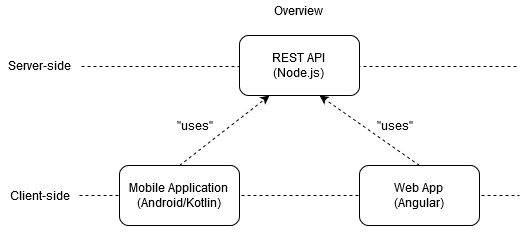
\includegraphics[scale=.8]{architecture}
	\caption{Modelo de arquitetura}
\end{figure}


\subsection{REST API}
A REST API, definida como primeira fase do projeto, constituirá o \textit{server-side} do mesmo. É pretendido que este módulo seja completamente independente dos outros, tendo como responsabilidade trabalhar como fonte de dados para os outros componentes (client-side). \par \medskip 

A tecnologia utilizada para desenvolver este componente será Node.js em conjunto com vários packages do NPM (node package manager), como o Express e o Passport. Esta escolha foi justificada por múltiplas razões:
\begin{itemize}
	\item domínio dos autores na linguagem Javascript e em vários módulos do NPM;
	\item popularidade da ferramenta, algo que simplifica o processo de desenvolvimento do componente devido à grande quantidade de recursos sobre a mesma;
	\item existência de suporte neste meio de execução de ferramentas para auxiliar o acesso à base de dados escolhida.
\end{itemize}
\par \medskip

O servidor será também responsável por hospedar a base de dados, que irá funcionar no motor MongoDB. A escolha deste serviço foi efetuada devido à fácil integração do mesmo com Node.js e devido ao facto deste ter um modelo de dados baseado em documentos JSON, algo que simplifica a inserção e pesquisa sobre os mesmos.
\par \medskip

\subsection{Aplicação \textit{Mobile}}
A aplicação \textit{mobile} será desenvolvida para a plataforma Android em Kotlin. A mesma irá seguir os princípios definidos pelo Android Jetpack, que disponibiliza ferramentas e bibliotecas cujas auxiliam o desenvolvimento da aplicação. As razões que levaram a esta decisão foram:
\begin{itemize}
	\item familiaridade dos autores com esta linguagem de programação e ferramentas(Android Jetpack);
	\item a nível de quota de mercado dos sistemas operativos de dispositivos móveis, o Android é o mais prevalente;
	\item atualmente, o Kotlin é a linguagem oficial para desenvolvimento de aplicações móveis para Android.
\end{itemize}

\subsection{Aplicação \textit{Web}}
A aplicação \textit{web} será desenvolvida em React. Esta tecnologia foi escolhida devido a:

\begin{itemize}
	\item familiaridade dos autores com esta ferramenta;
	\item quota de mercado (relativamente às frameworks de Javascript utilizadas para o desenvolvimento de aplicações \textit{web}) significativa, sendo atualmente a tecnologia mais usada;
	\item integração com as outras ferramentas do projeto.
\end{itemize}

\subsection{Tecnologias e ferramentas}
As seguintes tecnologias irão ser utilizadas durante o desenvolvimento do projeto:
\begin{itemize}
	\item \textbf{Javascript}: Principal linguagem para programação client-side em browsers; Esta é tipicamente utilizada em conjunto com ferramentas como o HTML e CSS para implementar a funcionalidade de uma página web;
	\item \textbf{Node.js}: Interpretador e ambiente de execução para Javascript normalmente utilizado para executar código sem ser num cliente browser;
	\item \textbf{NPM}: package manager do Javascript/Node.js;
	\item \textbf{Express}: web framework para Node.js. Auxilia o processo de routing e definição de endpoints, encapsulando aspetos do HTTP, para tornar mais fácil o desenvolvimento de \textit{Web} APIs;
	\item \textbf{Passport}: Middleware de autenticação usado em conjunto com o Express para simplificar o processo de autenticação e gestão de sessões de utilizadores;
	\item \textbf{MongoDB}: Base de dados noSQL baseada em documentos JSON. Tipicamente integrada com Javascript devido à natureza dos seus documentos;
	\item \textbf{Android}: Sistema operativo open source para dispositivos móveis desenvolvido pela Google. Atualmente, cerca de 75\% dos dispositivos móveis usam este SO;
	\item \textbf{Kotlin}: Linguagem de programação desenvolvida pela JetBrains que compila para a JVM. Atualmente, o Kotlin é a linguagem oficial do Android;
	\item \textbf{Android Jetpack}: Conjunto de ferramentas e bibliotecas as quais auxiliam a implementação e desenvolvimento de software para o sistema operativo móvel Android;
	\item \textbf{React}: Biblioteca \textit{open-source} de Javascript usada para desenvolver a UI de aplicações.
\end{itemize}